\documentclass[12pt, oneside]{article}

\usepackage[letterpaper, scale=0.89, centering]{geometry}
\usepackage{fancyhdr}
\setlength{\parindent}{0em}
\setlength{\parskip}{1em}

\usepackage{tikz}
\usetikzlibrary{automata,positioning,arrows}

\pagestyle{fancy}
\fancyhf{}
\renewcommand{\headrulewidth}{0pt}
\rfoot{\href{https://creativecommons.org/licenses/by-nc-sa/2.0/}{CC BY-NC-SA 2.0} Version \today~(\thepage)}

\usepackage{amssymb,amsmath,pifont,amsfonts,comment,enumerate,enumitem}
\usepackage{currfile,xstring,hyperref,tabularx,graphicx,wasysym}
\usepackage[labelformat=empty]{caption}
\usepackage{xcolor}
\usepackage{multicol,multirow,array,listings,tabularx,lastpage,textcomp,booktabs}

\lstnewenvironment{algorithm}[1][] {   
    \lstset{ mathescape=true,
        frame=tB,
        numbers=left, 
        numberstyle=\tiny,
        basicstyle=\rmfamily\scriptsize, 
        keywordstyle=\color{black}\bfseries,
        keywords={,procedure, div, for, to, input, output, return, datatype, function, in, if, else, foreach, while, begin, end, }
        numbers=left,
        xleftmargin=.04\textwidth,
        #1
    }
}
{}

\newcommand\abs[1]{\lvert~#1~\rvert}
\newcommand{\st}{\mid}

\newcommand{\cmark}{\ding{51}}
\newcommand{\xmark}{\ding{55}}
 
\begin{document}
\begin{flushright}
    \StrBefore{\currfilename}{.}
\end{flushright} \section*{Week2 friday}
{\bf Warmup}: Design a DFA (deterministic finite automaton) and an NFA (nondeterministic
finite automaton) that each recognize each of the following languages over $\{a,b\}$
\[
    \{ w \mid \text{$w$ has an $a$ and ends in $b$}\}
\]

\vfill

\[
    \{ w \mid \text{$w$ has an $a$ or ends in $b$}\}
\]

\vfill



\textbf{Strategy}: To design DFA or NFA for a given language,  
identify patterns that can be built up as we process strings and create states
for intermediate stages. Or: decompose the language to a simpler one 
that we already know how to recognize with a DFA or NFA.


{\it Recall} (from Wednesday of last week, and in textbook Exercise 1.14): 
if there is a DFA $M$ such that $L(M) = A$ then there is another DFA, let's call it $M'$, such that 
$L(M') = \overline{A}$, the complement of $A$, defined as $\{ w \in \Sigma^* \mid w \notin A \}$.


Let's practice defining automata constructions by coming up with other ways to get new automata from old.
\newpage

Suppose $A_1, A_2$ are languages over an alphabet $\Sigma$.
{\bf Claim:} if there is a NFA $N_1$ such that $L(N_1) = A_1$ and 
NFA $N_2$ such that $L(N_2) = A_2$, then there is another NFA, let's call it $N$, such that 
$L(N) = A_1 \cup A_2$.

{\bf Proof idea}: Use nondeterminism to choose which of $N_1$, $N_2$ to run.

\vfill
\begin{comment}
    Draw schematic
\end{comment}

{\bf Formal construction}: Let 
$N_1 = (Q_1, \Sigma, \delta_1, q_1, F_1)$ and $N_2 = (Q_2, \Sigma, \delta_2,q_2, F_2)$
and assume $Q_1 \cap Q_2 = \emptyset$ and that $q_0 \notin Q_1 \cup Q_2$.
Construct $N = (Q, \Sigma, \delta, q_0, F_1 \cup F_2)$ where
\begin{itemize}
    \item $Q = $
    \item $\delta: Q \times \Sigma_\varepsilon \to \mathcal{P}(Q)$ is defined by, for $q \in Q$ and $x \in \Sigma_{\varepsilon}$:
        \[
            \phantom{\delta((q,x))=\begin{cases}  \delta_1 ((q,x)) &\qquad\text{if } q\in Q_1 \\ \delta_2 ((q,x)) &\qquad\text{if } q\in Q_2 \\ \{q1,q2\} &\qquad\text{if } q = q_0, x = \varepsilon \\ \emptyset\text{if } q= q_0, x \neq \varepsilon \end{cases}}
        \]
\end{itemize}


\vfill
{\it Proof of correctness would prove that $L(N) = A_1 \cup A_2$ by considering
an arbitrary string accepted by $N$, tracing an accepting computation of $N$ on it, and using 
that trace to prove the string is in at least one of $A_1$, $A_2$; then, taking an arbitrary 
string in $A_1 \cup A_2$ and proving that it is accepted by $N$. Details left for extra practice.}


{\bf Example}: The language recognized by the NFA over $\{a,b\}$ with state diagram


    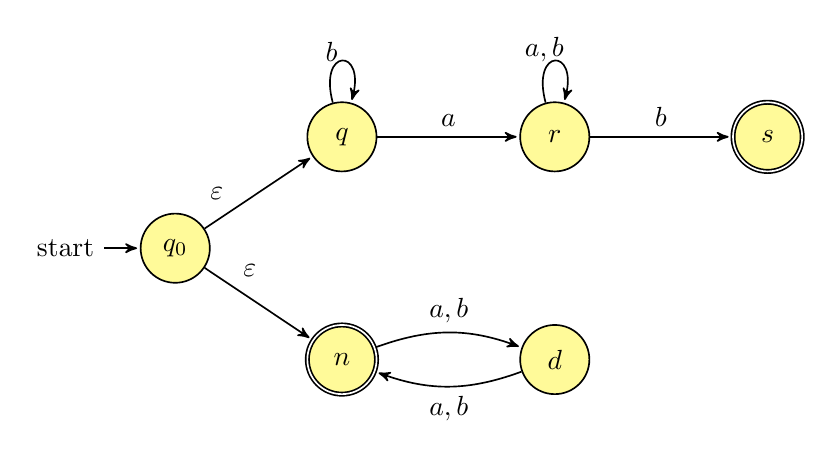
\begin{tikzpicture}[->,>=stealth',shorten >=1pt, auto, node distance=2cm, semithick]
    \tikzstyle{every state}=[text=black, fill=yellow!40]
    
    \node[initial,state] (q0)          {$q_0$};
    \node[state]         (q) [above right of=q0, xshift=20pt] {$q$};
    \node[state]         (r) [right of=q, xshift=20pt] {$r$};
    \node[state, accepting]         (s) [right of=r, xshift=20pt] {$s$};
    \node[state, accepting]         (n) [below right of=q0, xshift=20pt] {$n$};
    \node[state]         (d) [right of=n, xshift=20pt] {$d$};
    
    \path (q0) edge  [bend left=0, near start] node {$\varepsilon$} (q)
            edge [bend right=0, near start] node {$\varepsilon$} (n)
        (q) edge [bend left=0] node {$a$} (r)
            edge [loop above, near start] node {$b$} (q)
        (r) edge [bend left=0] node {$b$} (s)
            edge [loop above, near start] node {$a,b$} (r)
        (n) edge [bend left=20] node {$a,b$} (d)
        (d) edge [bend left=20] node {$a,b$} (n)
    ;
    \end{tikzpicture}
is:


\newpage

Could we do the same construction with DFA?

\vspace{50pt}

Happily, though, an analogous claim is true!

Suppose $A_1, A_2$ are languages over an alphabet $\Sigma$.
{\bf Claim:} if there is a DFA $M_1$ such that $L(M_1) = A_1$ and 
DFA $M_2$ such that $L(M_2) = A_2$, then there is another DFA, let's call it $M$, such that 
$L(M) = A_1 \cup A_2$. {\it Theorem 1.25 in Sipser, page 45}
    
    {\bf Proof idea}:
    
    
    {\bf Formal construction}: 
    
    \vfill

    
    {\bf Example}:  When $A_1 = \{w \mid w~\text{has an $a$ and ends in $b$} \}$ and 
    $A_2 = \{ w \mid w~\text{is of even length} \}$.
    
    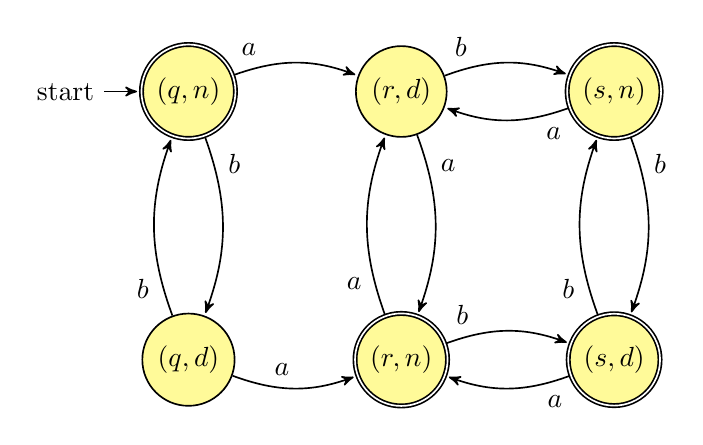
\begin{tikzpicture}[->,>=stealth',shorten >=1pt, auto, node distance=2cm, semithick]
        \tikzstyle{every state}=[text=black, fill=yellow!40]
        
        \node[initial,state,accepting] (qn)          {$(q,n)$};
        \node[state]         (qd) [below of=qn, yshift=-40pt] {$(q,d)$};
        \node[state]         (rd) [right of=qn, xshift=20pt] {$(r,d)$};
        \node[state,accepting]         (rn) [right of=qd, xshift=20pt] {$(r,n)$};
        \node[state,accepting]         (sn) [right of=rd, xshift=20pt] {$(s,n)$};
        \node[state,accepting]         (sd) [right of=rn, xshift=20pt] {$(s,d)$};
        
        \path (qn) edge  [bend left=20, near start] node {$b$} (qd)
                edge [bend left=20, near start] node {$a$} (rd)
            (qd) edge [bend left=20, near start] node {$b$} (qn)
                edge [bend right=20, near start] node {$a$} (rn)
            (rn) edge [bend left=20, near start] node {$a$} (rd)
                edge [bend left=20, near start] node {$b$} (sd)
            (rd) edge [bend left=20, near start] node {$a$} (rn)
                edge [bend left=20, near start] node {$b$} (sn)
            (sn) edge [bend left=20, near start] node {$a$} (rd)
                edge [bend left=20, near start] node {$b$} (sd)
            (sd) edge [bend left=20, near start] node {$a$} (rn)
                edge [bend left=20, near start] node {$b$} (sn)
        ;
        \end{tikzpicture}
    
    \newpage
    
    Suppose $A_1, A_2$ are languages over an alphabet $\Sigma$.
    {\bf Claim:} if there is a DFA $M_1$ such that $L(M_1) = A_1$ and 
    DFA $M_2$ such that $L(M_2) = A_2$, then there is another DFA, let's call it $M$, such that 
    $L(M) = A_1 \cap A_2$.  {\it Sipser Theorem 1.25, page 45}
    
    {\bf Proof idea}:
    
    
    {\bf Formal construction}: 
    
    \vspace{70pt}


    
 \vfill
\end{document}